\documentclass[oneside]{book}

% ----------------------
% Language and Encoding
% ----------------------
\usepackage{fontspec}
\usepackage{luatexja}
\usepackage{luatexja-fontspec}
\setmainjfont{Noto Serif CJK JP}

% ----------------------
% Mathematics (Legacy-Compatible)
% ----------------------
\usepackage{amsmath, amssymb, amsthm, mathtools, mathpartir}
\usepackage{tikz}
\usepackage{tikz-cd}

% ----------------------
% General Formatting
% ----------------------
\usepackage{graphicx}
\usepackage{geometry}
\usepackage{indentfirst}
\usepackage{hyperref}
\usepackage{enumerate}
\usepackage{tabularx}
\usepackage{cancel}
\usepackage{comment}
\usepackage{hyphenat}
\usepackage{ellipsis}
\usepackage{paracol}
\usepackage{xcolor}
\usepackage[most]{tcolorbox}

% ----------------------
% Logic (Proofs)
% ----------------------
\usepackage{fitch}
\usepackage{proof}

% ----------------------
% Math Shortcuts
% ----------------------
\newcommand*\Implies{\mathrel{\Rightarrow}}
\renewcommand*\implies{\mathrel{\rightarrow}}
\newcommand*\Iff{\mathrel{\Leftrightarrow}}
\renewcommand*\iff{\mathrel{\leftrightarrow}}
\renewcommand*\land{\mathrel{\&}}
\newcommand*\ex{\mathrel{\downarrow}}

\DeclareMathOperator{\sgn}{sgn}
\DeclareMathOperator{\lcm}{lcm}
\DeclareMathOperator{\mmc}{mmc}
\DeclareMathOperator{\mdc}{mdc}
\DeclareMathOperator{\erf}{erf}
\DeclareMathOperator{\ifc}{if}
\let\Re\relax
\DeclareMathOperator{\Re}{Re}
\let\Im\relax
\DeclareMathOperator{\Im}{Im}

\renewcommand*\d{\mathrm{d}}

% Sets
\newcommand*\N{\mathbb{N}}
\newcommand*\Z{\mathbb{Z}}
\newcommand*\Q{\mathbb{Q}}
\newcommand*\R{\mathbb{R}}
\newcommand*\C{\mathbb{C}}
\newcommand*\F{\mathbb{F}}

% Other math utils
\newcommand*{\mbb}[1]{\mathbb{#1}}
\newcommand*{\mcl}[1]{\mathcal{#1}}
\newcommand*{\mfr}[1]{\mathfrak{#1}}
\newcommand*{\floor}[1]{\left\lfloor#1\right\rfloor}
\newcommand*{\ceil}[1]{\left\lceil#1\right\rceil}
\renewcommand*\O{\mathcal{O}}
\renewcommand*\emptyset{\varnothing}
\newcommand*\df{\mathrm{df}}

\everymath{\displaystyle}

% ----------------------
% Links
% ----------------------
\hypersetup{
    bookmarksnumbered=true,
    colorlinks=true,
    linkcolor=black,
    citecolor=black,
    urlcolor=blue,
}

% ----------------------
% Playing card symbols
% ----------------------
\DeclareSymbolFont{extraup}{U}{zavm}{m}{n}
\DeclareMathSymbol{\spades}{\mathalpha}{extraup}{81}
\DeclareMathSymbol{\clubs}{\mathalpha}{extraup}{84}
\DeclareMathSymbol{\hearts}{\mathalpha}{extraup}{86}
\DeclareMathSymbol{\diamonds}{\mathalpha}{extraup}{87}

% ----------------------
% Fix \pmod*
% ----------------------
\makeatletter
\let\@@pmod\pmod
\DeclareRobustCommand{\pmod}{\@ifstar\@pmods\@@pmod}
\def\@pmods#1{\mkern4mu({\operator@font mod}\mkern 6mu#1)}
\makeatother

% ----------------------
% Better \widebar
% ----------------------
\makeatletter
% (Seu código customizado para widebar pode entrar aqui se quiser manter. Omiti por brevidade.)
\makeatother

% ----------------------
% Documento
% ----------------------
\title{Mathematica Collectanea}
\author{eyeS}
\date{March 2025}

% Vintage Parchment Theme
% Inspired by the soft yellow tones of old paper.

\usepackage{xcolor}
\usepackage{pagecolor}

% Soft parchment-like background
\definecolor{parchment}{RGB}{250, 245, 229}   % light yellow-beige
\definecolor{textblack}{RGB}{30, 30, 30}      % dark grayish text

\pagecolor{parchment}
\color{textblack}


\begin{document}

\begin{titlepage}
    \centering
    \vspace*{3cm}
    {\Huge \bfseries Physics Collectanea \par}
    \vspace{0.5cm}
    {\large A Personal Compendium of Physics Notes\par}
    \vfill
    {\LARGE \bfseries eyeS\par}
    \vspace{0.5cm}
    {\Large \textsc{March 2025}}
\end{titlepage}

\tableofcontents
\clearpage

% Notes content
\part{Condensed Matter}
\chapter{Basic Models of Metals}

\section{The Drude Model}


\begin{figure}[htbp]
  \centering
  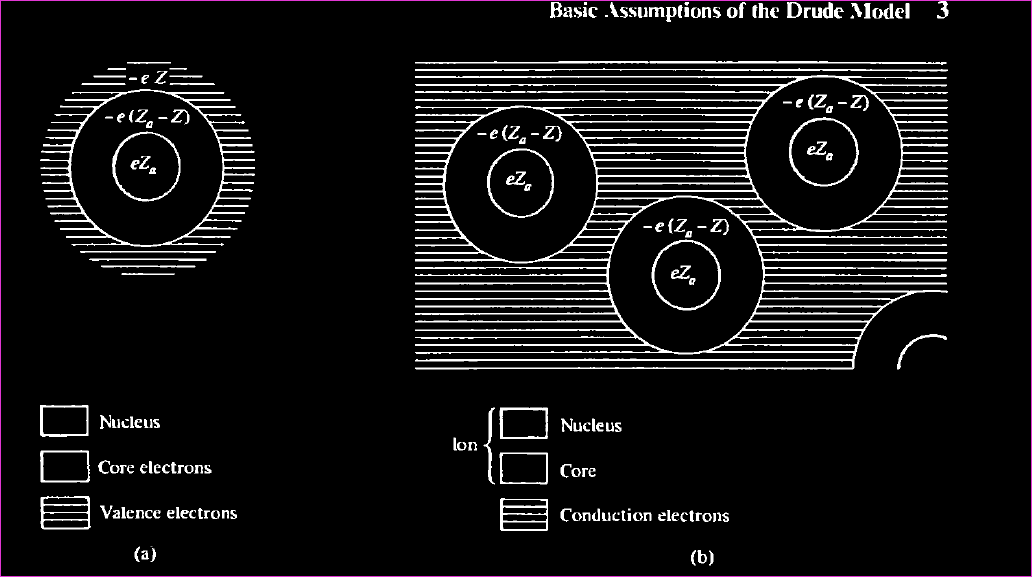
\includegraphics[width=\linewidth]{images/basic_assumptions.png}
\end{figure}

The Drude model assumes that we have immovable nucleus with most extern electons free. A nucleus of some element, has $Z$ protons, and subsequently $Z$ electrons with total charge $-eZ$. 

Let's try to derive somethings. We know that electrical force $\vec{F} = -e\vec{E}$ and $\vec{F} = m\vec{a}$. Thus we have:

\begin{equation}
  \vec{a} = \frac{-eE}{m}
\end{equation}

After a collision, the electron accelerates for a time $t$, gaining velocity:

\begin{equation}
  \Delta{\vec{v}} = \vec{a}\cdot t = \frac{-eEt}{m}
\end{equation}

So the final velocity is:

\begin{equation}
  \vec{v}(t) = \vec{v_0}(t) + \Delta{\vec{v}}
\end{equation}

Well, we assume that the collision randomize \textbf{$\vec{v_0}$} (it's isotropic), its \textbf{average is zero}:

$$
  \langle\vec{v_0}\rangle = 0 \implies \langle\vec{v}(t)\rangle = \frac{-eE\langle t \rangle}{m} $$

We know that $\textbf{j} = -ne\textbf{v}$, so we have:

\begin{equation}
  \textbf{j} = -nev_{avg} = -ne\left(\frac{-eE\tau}{m}\right) = \left(\frac{ne²\tau}{m}\right)E
\end{equation}

Let's define the \textbf{conductivity} ($\sigma$) that tell us how easily a material allows electric charges to move when you apply an electric field (that's created when you make a differential in potential). Then:

\begin{equation}
  \textbf{j} = \sigma \textbf{E}
\end{equation}

Notice that conductivity is the inverse of resistivity:

\begin{equation}
  \sigma = \frac{1}{\rho}
\end{equation}

We can determine the relaxation time $\tau$ usgin the resistivity:

\begin{equation}
  \tau = \frac{m}{\rho ne^2}
\end{equation}

\input{text/soft_condensed_matter.tex}
\end{document}

